\documentclass[10pt]{article}
\usepackage[letterpaper,textwidth=181mm,top=20mm,bottom=20mm]{geometry}
\usepackage[T1]{fontenc}
\usepackage{amsmath,amssymb}
\usepackage{tikz}
\usetikzlibrary{arrows.meta,positioning,calc,fit,backgrounds,shapes.geometric}
\usepackage{pgfplots}
\pgfplotsset{compat=1.17}
\usepgfplotslibrary{groupplots}
\usepackage{caption}
\captionsetup{font=small,labelfont=bf}
\pagestyle{empty}
\definecolor{cProp}{HTML}{1D60BC}
\definecolor{cEM}{HTML}{A388D2}
\definecolor{cSQ}{HTML}{ED914C}
\definecolor{cDA}{HTML}{47C496}
\definecolor{cInk}{HTML}{3A3A3A}
\definecolor{cMuted}{HTML}{8A8A8A}
\pgfplotsset{
  every axis/.append style={
    font=\small, tick label style={font=\footnotesize}, label style={font=\small},
    legend style={font=\footnotesize, draw=none, fill=none, cells={anchor=west}},
    axis line style={cInk!60}, tick style={cInk!60},
    major grid style={black!8}, ymajorgrids,
    width=0.48\textwidth, height=5.2cm, xtick pos=bottom, ytick pos=left,
  },
  mProp/.style={cProp, solid, line width=1.2pt, mark=*, mark size=1.5pt, mark options={solid, fill=cProp}},
  mEM/.style={cEM, densely dotted, line width=1.0pt, mark=triangle*, mark size=1.8pt, mark options={solid, fill=white}},
  mSQ/.style={cSQ, dashed, line width=1.0pt, mark=square*, mark size=1.3pt, mark options={solid, fill=white}},
  mDA/.style={cDA, dash dot, line width=1.0pt, mark=diamond*, mark size=1.8pt, mark options={solid, fill=white}},
  bProp/.style={fill=cProp, draw=white, line width=0.4pt, area legend},
  bEM/.style={fill=cEM, draw=white, line width=0.4pt, area legend},
  bSQ/.style={fill=cSQ, draw=white, line width=0.4pt, area legend},
  bDA/.style={fill=cDA, draw=white, line width=0.4pt, area legend},
  refline/.style={black!40, thin, densely dashed},
}
\newcommand{\tenexp}[1]{$10^{\mbox{\footnotesize$#1$}}$}

\newcommand{\column}[1]{\begin{minipage}{88.9mm}\centering #1\end{minipage}}
\begin{document}

\begin{figure}[h]
\centering
\column{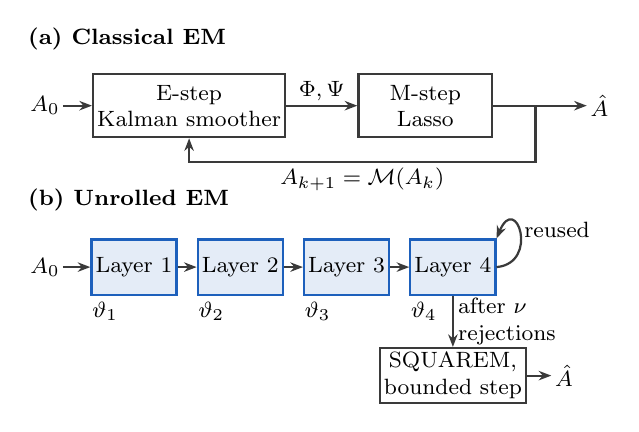
\begin{tikzpicture}[
  font=\footnotesize, >={Stealth[length=1.6mm]},
  blk/.style={draw=cInk, thick, minimum height=8mm, align=center, inner sep=1.5pt},
  lrn/.style={blk, draw=cProp, fill=cProp!12, minimum width=10.6mm, minimum height=7mm},
  lab/.style={font=\footnotesize\bfseries, anchor=west, inner sep=0pt},
  line/.style={->, draw=cInk, thick},
]
\node[lab] at (0,0.85) {(a) Classical EM};
\node[blk, minimum width=21mm] (e) at (2.05,0) {E-step\\Kalman smoother};
\node[blk, minimum width=17mm] (m) at (5.05,0) {M-step\\Lasso};
\node[inner sep=1pt] (a0) at (0.22,0) {$A_0$};
\draw[line] (a0) -- (e);
\draw[line] (e) -- node[midway, above, inner sep=1.5pt] {$\Phi,\Psi$} (m);
\draw[line] (m) -- (7.1,0) node[right, inner sep=1pt] {$\hat A$};
\draw[line] (6.45,0) -- (6.45,-0.72) -- node[below, inner sep=1.5pt] {$A_{k+1}=\mathcal{M}(A_k)$} (2.05,-0.72) -- (e.south);
\begin{scope}[yshift=-2.05cm]
\node[lab] at (0,0.85) {(b) Unrolled EM};
\node[inner sep=1pt] (b0) at (0.22,0) {$A_0$};
\node[lrn] (l1) at (1.35,0) {Layer 1};
\node[lrn] (l2) at (2.70,0) {Layer 2};
\node[lrn] (l3) at (4.05,0) {Layer 3};
\node[lrn] (l4) at (5.40,0) {Layer 4};
\draw[line] (b0) -- (l1);
\draw[line] (l1) -- (l2);
\draw[line] (l2) -- (l3);
\draw[line] (l3) -- (l4);
\foreach \i in {1,2,3,4} {\node[below=0.6mm of l\i.south west, anchor=north west, inner sep=0.5pt] {$\vartheta_\i$};}
\draw[line] (l4.east) .. controls +(0.55,0.05) and +(0.25,0.6) .. (l4.north east) node[pos=0.55, right, inner sep=1.5pt] {reused};
\node[blk, minimum width=17mm, minimum height=7mm, below=6.5mm of l4] (sq) {SQUAREM,\\bounded step};
\draw[line] (l4) -- node[midway, right, inner sep=1.5pt, align=left] {after $\nu$\\rejections} (sq);
\draw[line] (sq) -- ++(1.25,0) node[right, inner sep=1pt] {$\hat A$};
\end{scope}
\end{tikzpicture}
}
\caption{Classical EM and the unrolled EM algorithm with handover to SQUAREM.}
\end{figure}

\begin{figure}[h]
\centering
\begin{tikzpicture}
\begin{groupplot}[group style={group size=2 by 1, horizontal sep=17mm},
  width=0.475\textwidth, height=4.0cm, xmin=0, xmax=60, xlabel={number of E-steps},
  every axis plot/.append style={mark size=1.3pt}, unbounded coords=jump]
\nextgroupplot[ymode=log, ymin=5e-10, ymax=0.3,
  ytick={1e-9,1e-7,1e-5,1e-3,1e-1}, yticklabels={\tenexp{-9},\tenexp{-7},\tenexp{-5},\tenexp{-3},\tenexp{-1}}, yminorticks=false,
  ylabel={relative objective gap},
  legend to name=traceleg, legend columns=4, legend style={/tikz/every even column/.append style={column sep=3mm}}]
\addplot[mProp, mark repeat=4] table[x=e,y=g] {data/distR_prop.csv};
\addplot[mEM, mark repeat=4] table[x=e,y=g] {data/distR_em.csv};
\addplot[mSQ, mark repeat=4] table[x=e,y=g] {data/distR_sq.csv};
\addplot[mDA, mark repeat=4, mark phase=2] table[x=e,y=g] {data/distR_da.csv};
\legend{Proposed, EM, SQUAREM, DAAREM}
\draw[black!40, thin, densely dashed] (axis cs:16,5e-10) -- (axis cs:16,0.3);
\nextgroupplot[ymode=log, ymin=5e-5, ymax=2, ytick={1e-4,1e-3,0.01,0.1,1}, yticklabels={\tenexp{-4},\tenexp{-3},0.01,0.1,1}, yminorticks=false,
  ylabel={relative distance to reference}]
\addplot[mProp, mark repeat=4] table[x=e,y=d] {data/distR_prop.csv};
\addplot[mEM, mark repeat=4] table[x=e,y=d] {data/distR_em.csv};
\addplot[mSQ, mark repeat=4] table[x=e,y=d] {data/distR_sq.csv};
\addplot[mDA, mark repeat=4, mark phase=2] table[x=e,y=d] {data/distR_da.csv};
\addplot[refline, forget plot] coordinates {(0,0.01) (60,0.01)};
\draw[black!40, thin, densely dashed] (axis cs:16,5e-5) -- (axis cs:16,2);
\end{groupplot}
\node[font=\small, anchor=north] at ($(group c1r1.south)+(0,-0.85cm)$) {(a) Objective gap};
\node[font=\small, anchor=north] at ($(group c2r1.south)+(0,-0.85cm)$) {(b) Distance to the reference solution};
\node[anchor=north] at ($(group c1r1.south)!0.5!(group c2r1.south)+(0,-1.35cm)$) {\pgfplotslegendfromname{traceleg}};
\end{tikzpicture}

\caption{Convergence on a typical F128 test system; the dashed line marks the handover to SQUAREM, and negative gaps are not shown.}
\end{figure}

\begin{figure}[h]
\centering
\column{\begin{tikzpicture}
\begin{axis}[width=\linewidth, height=3.8cm,
  xtick={0,...,6}, xticklabels={2,1.5,1.2,1.1,1.05,1.02,1.01}, xmin=-0.3, xmax=6.3,
  ymode=log, ymin=1.5, ymax=80, ytick={2,5,10,20,50}, yticklabels={2,5,10,20,50}, yminorticks=false,
  xlabel={accuracy target $\alpha$}, ylabel={median E-steps},
  legend style={at={(0.5,1.03)}, anchor=south, /tikz/every even column/.append style={column sep=3mm}}, legend columns=2]
\addplot[mProp] table[x=i,y=prop] {data/tol_F128.csv};
\addplot[mEM] table[x=i,y=em] {data/tol_F128.csv};
\addplot[mSQ] table[x=i,y=sq] {data/tol_F128.csv};
\addplot[mDA] table[x=i,y=da] {data/tol_F128.csv};
\legend{Proposed, EM, SQUAREM, DAAREM}
\end{axis}
\end{tikzpicture}
}
\caption{Median number of E-steps versus the accuracy target $\alpha$ for F128.}
\end{figure}

\begin{figure}[h]
\centering
\column{\begin{tikzpicture}
\begin{axis}[width=\linewidth, height=4.4cm, ybar=0pt, bar width=4.2pt, xtick=data, xticklabels from table={data/motiv_steps.csv}{setting},
  xmin=-0.6, xmax=4.6, ymin=0, ymax=15, ytick={0,2,...,12}, enlarge x limits=false, ylabel={median step},
  legend style={at={(0.02,0.98)}, anchor=north west, fill=white, fill opacity=0.85, text opacity=1}, legend columns=2]
\addplot[fill=cMuted, draw=white, area legend] table[x=x, y=idd] {data/motiv_steps.csv};
\addplot[fill=cProp, draw=white, area legend] table[x=x, y=lrd] {data/motiv_steps.csv};
\addplot[fill=cMuted!40, draw=white, area legend] table[x=x, y=ido] {data/motiv_steps.csv};
\addplot[fill=cProp!40, draw=white, area legend] table[x=x, y=lro] {data/motiv_steps.csv};
\legend{ideal diag., learned diag., ideal off-diag., learned off-diag.}
\end{axis}
\end{tikzpicture}
}
\caption{Median ideal and learned first steps by class of entries.}
\end{figure}

\end{document}
